\section{RESULTADOS}

Siguiendo la metodología, los resultados se organizan en tres niveles: verificación del software (¿se construyó bien?), validación técnica del modelo (¿reproduce los datos de la encuesta?) y evaluación del cumplimiento de los requerimientos y los objetivos. Al final se declaran las limitaciones.

\subsection{Verificación del software}

\textbf{Pruebas automáticas.} El servicio tiene 103 pruebas con \texttt{pytest} en \texttt{simulation-service/test/}, que cubren: demanda y presets, generación de viajes, conversión del FCD, exportación a kepler, intersecciones, priorización, avance y cancelación, semáforo nuevo, escena 3D, telemetría, simulaciones precalculadas, la API y la comparación 3D. Las dependencias externas se aíslan con \texttt{dependency\_overrides} y datos mínimos, de modo que las pruebas no ejecutan SUMO completo. Entre ellas, una prueba verifica que el preset \textit{encuesta} con sus conteos por defecto reproduce exactamente la expansión simple de la encuesta, lo que valida la lógica de transferencia modal en su caso base.

Dos limitaciones de este nivel de verificación: (i) el flujo de integración continua instala solo el \texttt{requirements.txt} de la raíz y ejecuta un directorio de pruebas que es un marcador, por lo que \textbf{las pruebas del servicio se ejecutan manualmente} y no en cada cambio; y (ii) el visor no tiene pruebas automáticas, solo demostración funcional.

\textbf{Estado de los requerimientos.} La tabla~\ref{tab:estado-req} resume el estado de los 60 requerimientos del SRS al cierre del proyecto.

\begin{table}[ht]
\renewcommand{\arraystretch}{1.15}
\centering
\small
\begin{tabular}{|l|c|c|c|c|c|}
\hline
\textbf{Tipo} & \textbf{Total} & \textbf{Implementado / cumplido} & \textbf{Parcial} & \textbf{Pendiente} & \textbf{Otro} \\ \hline
Funcionales (RF) & 45 & 30 & 9 & 5 & 1 reemplazado \\ \hline
Desempeño (RD) & 4 & 2 & 0 & 0 & 1 no aplica, 1 por verificar \\ \hline
No funcionales (RNF) & 11 & 5 & 6 & 0 & 0 \\ \hline
\textbf{Total} & \textbf{60} & \textbf{37} & \textbf{15} & \textbf{5} & \textbf{3} \\ \hline
\end{tabular}
\caption{Estado de los requerimientos del SRS.}
\label{tab:estado-req}
\end{table}

Los cinco requerimientos funcionales pendientes son: la validación por GEH contra los aforos HMD (RF-014), la reanudación por \textit{checkpoint} (RF-016), el reporte exportable de la comparación 3D (RF-041), el programa editable del semáforo propuesto (RF-042) y el transporte público con buses y paradas reales (RF-043). El requerimiento reemplazado es la matriz O/D en formato \texttt{.od}, que se sustituyó por viajes TAZ (\texttt{fromTaz}/\texttt{toTaz}) que \texttt{duarouter} rutea directamente. Los parciales corresponden en su mayoría a la limpieza de datos, que se hace en los cuadernos de la Fase 2 y no en el servicio, a la validación del formulario web y a la mantenibilidad (documentación y CI). Los cuatro de desempeño: RD-001 y RD-003 cumplidos, RD-002 no aplica (la matriz se arma en los cuadernos) y RD-004 (30 cuadros por segundo) queda por verificar en la prueba de aceptación.

\subsection{Resultados de las simulaciones}

Los cuatro presets se simularon una vez con sus conteos por defecto, con la demanda completa de la encuesta (24.647 viajes en la ventana de 7:00 a 10:00). La tabla~\ref{tab:presets} resume la carga y la ejecución en SUMO.

\begin{table}[ht]
\renewcommand{\arraystretch}{1.15}
\centering
\small
\begin{tabular}{|l|r|r|r|r|r|r|}
\hline
\textbf{Preset} & \textbf{Viajes} & \textbf{Vehículos insertados} & \textbf{Personas cargadas} & \textbf{Teleports} & \textbf{Colisiones} & \textbf{Tamaño (MB)} \\ \hline
Encuesta & 24.647 & 9.592 & 14.123 & 209 & 80 & 11,7 \\ \hline
Más vehículos & 24.647 & 14.404 & 9.234 & 254 & 58 & 10,5 \\ \hline
Más peatones & 24.647 & 6.125 & 17.985 & 141 & 123 & 14,1 \\ \hline
Día sin carro & 24.647 & 4.945 & 19.257 & 106 & 134 & 16,0 \\ \hline
\end{tabular}
\caption{Resultados de las simulaciones precalculadas.}
\label{tab:presets}
\end{table}

Todos los presets conservan el total de viajes, y el sentido del cambio es el esperado: al pasar de \textit{más vehículos} a \textit{día sin carro}, los vehículos insertados bajan de 14.404 a 4.945 y las personas cargadas suben de 9.234 a 19.257. En el preset base se cargaron 10.324 vehículos y se insertaron 9.592 (92,9\,\%); el resto no pudo entrar a la red durante la ventana, lo que ocurre cuando el tramo de entrada está saturado. Los teletransportes (entre 106 y 254) y las colisiones (entre 58 y 134) son eventos del modelo de SUMO que se reportan, no se ocultan, y se discuten como limitación. Cabe notar que el mayor número de colisiones aparece en los presets con más peatones, no en el de más vehículos.

\textbf{Tiempo de ejecución.} Una corrida completa de la encuesta tarda unos 12 minutos: generación de demanda y \texttt{duarouter} unos 1,5, SUMO unos 8 y la exportación unos 2. Es muy inferior al límite de 4 horas del requerimiento RD-001 (cumplido). La preparación de una comparación 3D toma decenas de segundos, más 240~s simulados de calentamiento al conectarse.

\textbf{Tamaño de la salida.} La compresión del GeoJSON de la simulación base pasó de 63,7~MB a 11,7~MB (reducción del 81,6\,\%), lo que permite al navegador cargarlo con una barra de progreso.

\subsection{Validación frente a la encuesta}

Se comparó la distribución de la hora de salida de los viajes en intervalos de 10 minutos entre tres series (figura~\ref{fig:histograma}): la encuesta expandida por \texttt{fexp} ($n=109.372$), la encuesta tal como se entrega a SUMO ($n=24.647$, cada fila replicada $\mathrm{round}(f_{exp})$ veces con tope de 50) y la simulación base ($n=15.900$ viajes exportados).

\begin{figure}[H]
\centering
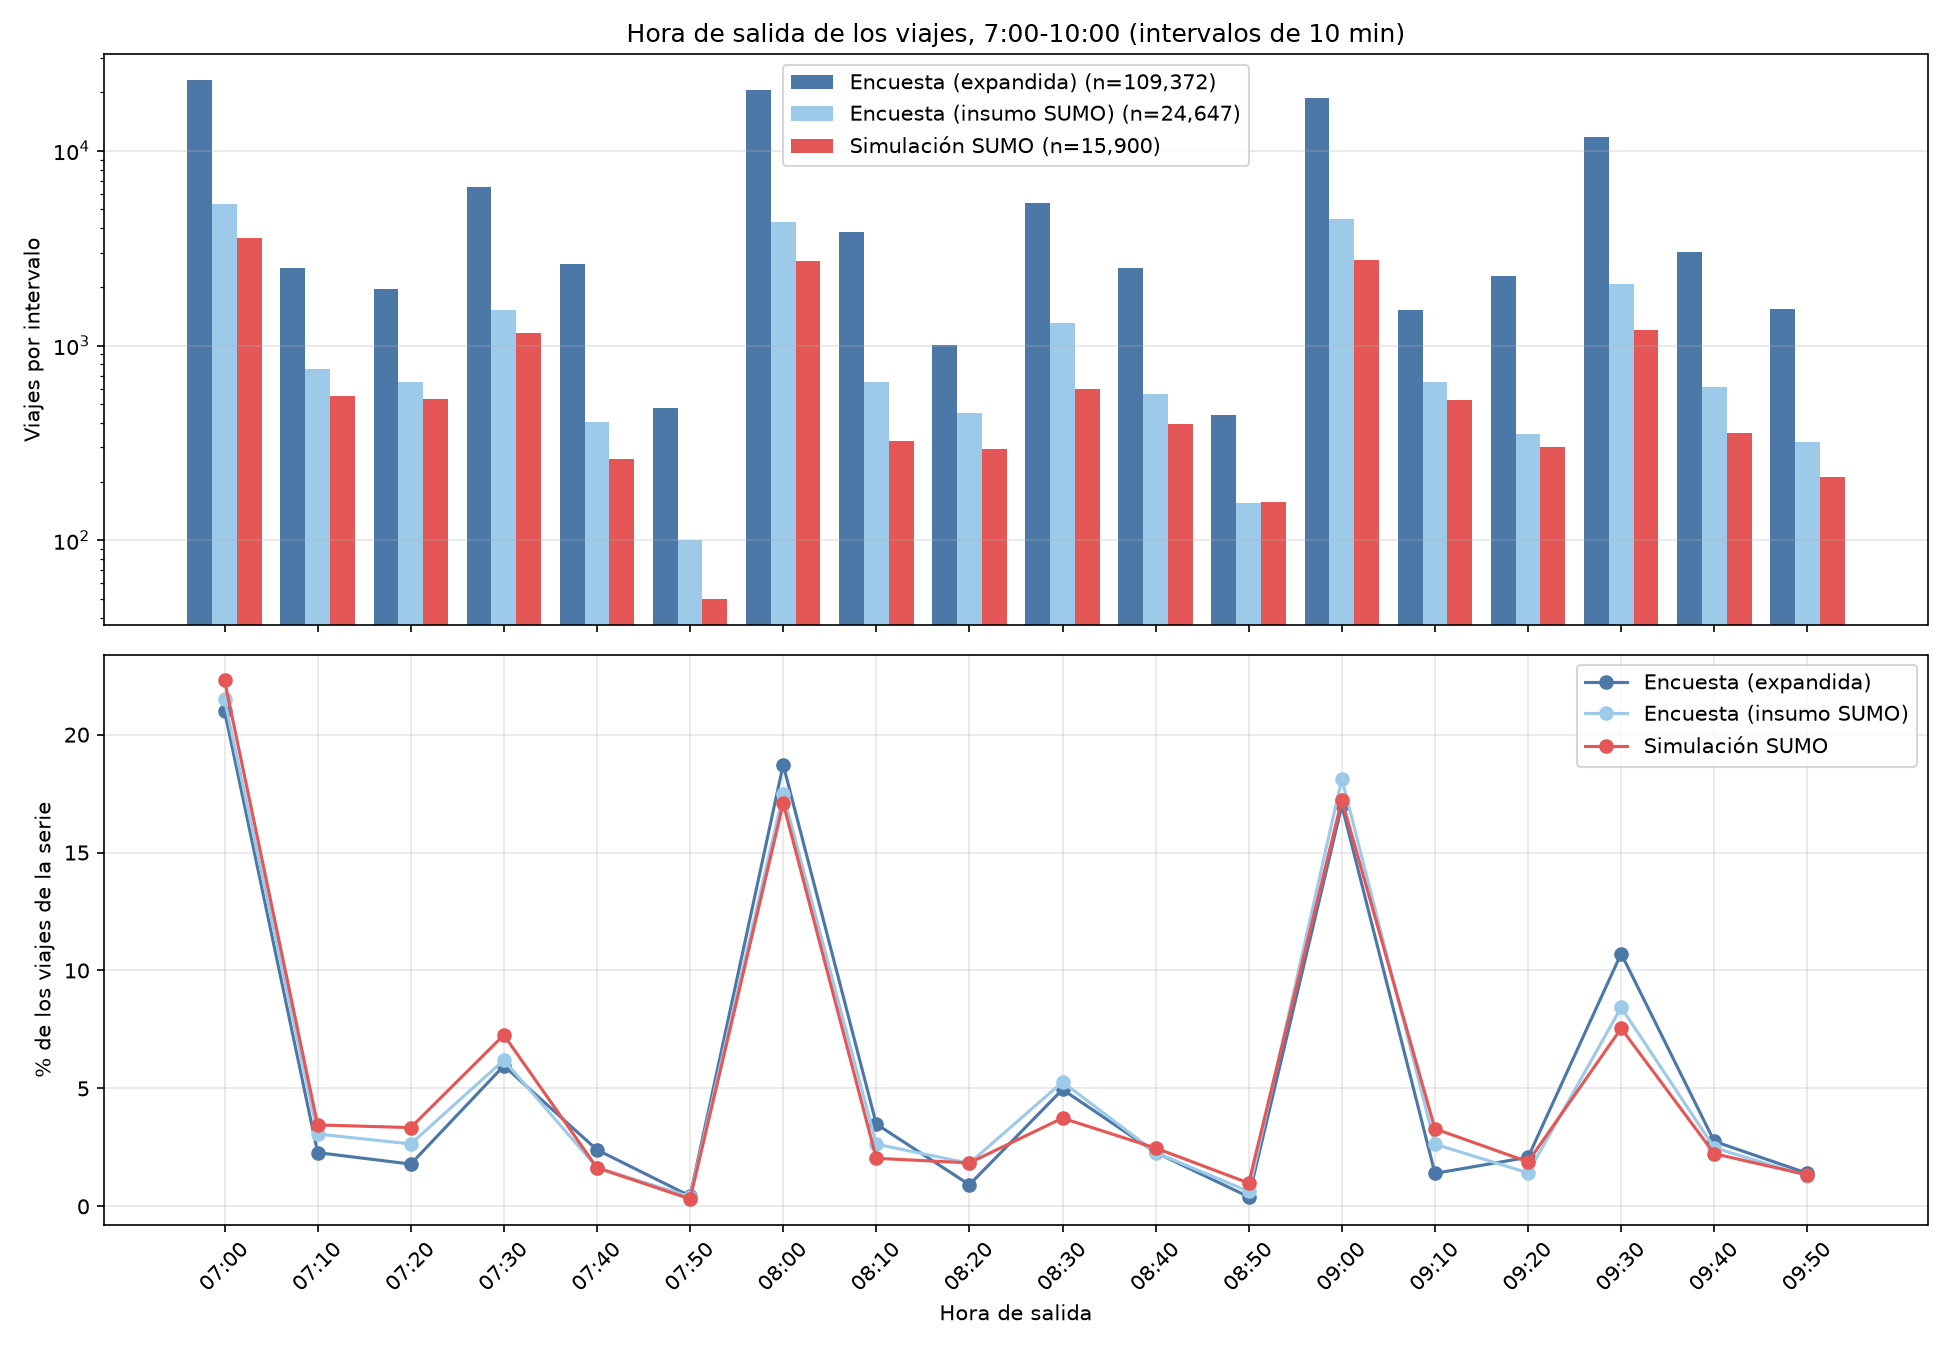
\includegraphics[width=\textwidth]{histograma_salidas.png}
\caption{Hora de salida de los viajes entre 7:00 y 10:00: encuesta expandida, encuesta como insumo de SUMO y simulación. Arriba, conteos (escala logarítmica); abajo, porcentaje de cada serie.}
\label{fig:histograma}
\end{figure}

El panel inferior, que normaliza cada serie para comparar solo la forma, muestra que las tres curvas siguen el mismo perfil: tres picos en las horas en punto (7:00, 8:00 y 9:00, que concentran cerca de 21\,\%, 18\,\% y 17\,\% de los viajes) y un pico menor a las 9:30. Los picos en horas exactas reflejan el redondeo con que los encuestados reportan su hora de salida, y la simulación los conserva. Las diferencias visibles son pequeñas: la simulación está algo por encima en las 7:30 y por debajo en las 9:30 (7,5\,\% frente a 10,7\,\% en la encuesta expandida).

Los totales distintos (109.372, 24.647 y 15.900) tienen explicaciones concretas. La expansión por \texttt{fexp} se acota a 50 copias por registro, y el exportador a kepler descarta las entidades que casi no se mueven y reduce los puntos de cada trayectoria. Por eso el histograma valida la \textbf{forma temporal} de la demanda, no su magnitud.

\subsection{Limitaciones y amenazas a la validez}
\label{sec:limitaciones-resultados}

\begin{itemize}[noitemsep]
    \item \textbf{No hay validación por GEH/RMSE.} Los aforos HMD no traen coordenadas, solo un texto libre de localización, y no se logró asociarlos a la red a tiempo. Por eso el criterio de la propuesta (GEH $<5$ en al menos 85\,\% de los puntos) \textbf{no se evaluó}. Los resultados de volumen son plausibles en su forma temporal, pero no están calibrados contra conteos reales. Es el principal pendiente del proyecto.
    \item \textbf{Transporte público como caminata.} No hay buses, paradas ni GTFS; se subestima la carga sobre las vías y se sobrestiman los peatones.
    \item \textbf{Programas semafóricos genéricos.} Los 220 semáforos usan el programa por defecto de \texttt{netconvert}, no los de la SDM. Por tanto, las comparaciones de programas son ilustrativas.
    \item \textbf{Tráfico de fondo sintético} en las comparaciones 3D, necesario porque la demanda real es escasa en una zona de 350~m. Los resultados dependen de las intensidades elegidas.
    \item \textbf{Una semilla.} El simulador 3D usa la semilla 42; no se hizo análisis de sensibilidad ni se repitió con varias semillas, por lo que los indicadores de riesgo de un actor son ilustrativos, no estadísticos.
    \item \textbf{Priorización sin validación externa.} La evidencia se calibró contra los semáforos ya existentes de la red, pero no se contrastó con una decisión real de la SDM ni con un conjunto independiente.
    \item \textbf{Ventana horaria y alcance.} Solo se simula la franja de 7:00 a 10:00 en Usaquén. Los datos crudos de la encuesta no se versionan, por lo que reproducir desde cero requiere el TSV filtrado.
    \item \textbf{Escena 3D parcialmente ilustrativa} (edificios de relleno marcados) y sin prueba de usuario: la usabilidad quedó \textit{implementada, pendiente de prueba con usuarios}.
\end{itemize}

\subsection{Cumplimiento de los objetivos}

\begin{table}[ht]
\renewcommand{\arraystretch}{1.15}
\centering
\small
\begin{tabular}{|p{1.8cm}|p{8cm}|p{4.2cm}|}
\hline
\textbf{Objetivo} & \textbf{Evidencia} & \textbf{Estado} \\ \hline
OE1 & Informe de brechas (Fase 1), selección del TSV de viajes internos y de la red OSM. & Cumplido, con las brechas de aforos declaradas. \\ \hline
OE2 & \textit{Pipeline} ETL de la encuesta a SUMO, con 103 pruebas. & Cumplido. \\ \hline
OE3 & Escenario de Usaquén ejecutado en SUMO y comparación de horas de salida contra la encuesta. & Parcial: sin GEH ni RMSE. \\ \hline
OE4 & Visor web con presets, parametrización, avance y cancelación. & Cumplido. \\ \hline
OE5 & Análisis de intersecciones y simulador 3D con TTC, DRAC y PET. & Cumplido; reporte exportable pendiente. \\ \hline
\end{tabular}
\caption{Cumplimiento de los objetivos específicos.}
\label{tab:objetivos}
\end{table}
